\section{Deep neural network and hyperparameter tuning}
\label{sec:deep-network}

\subsection{Network implementation}
We used a fully connected deep neural network (DNN) to classify students as
\texttt{Dropout} or \texttt{Graduate}. This suits tabular data. A CNN would assume
spatial relationships between columns that do not exist here. The network uses
103 inputs after preprocessing the original retained features, without the
extra engineered features. Its three hidden layers contain 128, 64 and 32
neurons, followed by two class outputs. In total, it learns 23,714 parameters.

ReLU allows nonlinear relationships. We trained with AdamW~\cite{loshchilov2019adamw},
weight decay 0.0001 and batches of 128 students. Weight decay discourages overly
large weights. A weighted classification loss gives both outcome classes equal importance.
In each training fit, the class weight is the training total divided by twice
that class's count. For the full-development fit this gives weight 0.822 for
Graduate (1,767 students) and 1.277 for Dropout (1,137 students).

\subsection{Tuning and justification}
Table~\ref{tab:dnn-search} lists the settings tested. Their combinations give
eight networks. Here, network dropout means randomly ignoring neurons during
training. This is unrelated to the student outcome.

\begin{table}[H]
\centering
\small
\caption[DNN tuning grid]{DNN settings tested and why they were varied.}
\label{tab:dnn-search}
\begin{tabularx}{\linewidth}{@{}l l X@{}}
\toprule
Setting & Values tested & Purpose \\
\midrule
Neurons per layer & (64, 32, 16) or (128, 64, 32) & Test whether a larger network learns useful patterns or overfits. \\
Learning rate & 0.001 or 0.0003 & Compare larger and smaller changes to the weights during training. \\
Network dropout & 0 or 0.3 & Test whether ignoring 30\% of neurons during training reduces overfitting. \\
\bottomrule
\end{tabularx}
\end{table}

The 2,904 development students were used for training and tuning. Each setting
was checked using five-fold cross-validation: train on four parts and validate
on the fifth, repeating for all five parts. We selected the highest mean
validation average precision (AP). AP measures how well dropout cases are
ranked above graduates. Higher is better, and it is not an accuracy
percentage~\cite{sklearn_ap}.
This selects the DNN configuration. The final model recommendation in Section~\ref{sec:transfer-comparison}
also considers contact-budget performance and explainability.

Within each training fit, one of seven stratified group folds determined the
training length, using split seed 42. Identical retained profiles stay together.
For the final development fit, this internal validation group has 415 students
(252 Graduate, 163 Dropout). The remaining 2,489 train the stopping-stage network.
Preprocessing was fitted without the internal validation group. Training stopped
after 12 epochs without improvement, with a limit of 120 epochs. An epoch is
one pass through the training data. We then trained a fresh network on all
available training rows for the selected number of epochs. The test set was
not used for these choices.

\subsection{Selected settings and results}
The selected network had 128, 64 and 32 neurons, learning rate 0.0003 and no
network dropout. Its mean AP across the five validation folds was 0.941.
All eight settings scored between 0.939 and 0.941, so tuning produced only
small differences (Figure~\ref{fig:dnn-tuning}). This does not establish one
clearly better architecture. The main search uses network seed 42.
At the selected settings, a development-only check with seeds 42, 7 and 2026
produced mean validation AP 0.9407, 0.9399
and 0.9379, respectively, on the same folds. Seed 42 is used for the reported
model. This checks initialization
sensitivity, not whether all architecture differences are robust.
The selected DNN's mean validation AP of 0.9407 is close to LDA's 0.9397.
This small difference alone does not justify preferring the more complex
network. Section~\ref{sec:final-evaluation} compares the DNN with the recommended LDA classifier.

\begin{figure}[H]
\centering
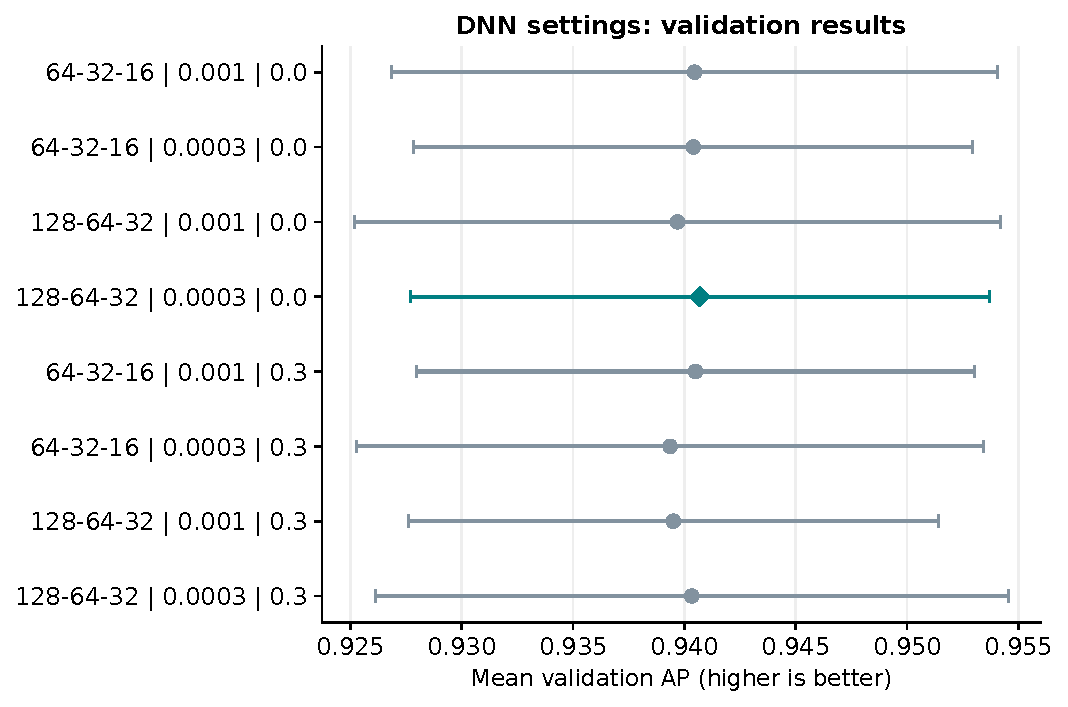
\includegraphics[width=0.82\linewidth]{Images/09_dnn_hyperparameter_comparison.pdf}
\caption[DNN validation AP across tuning settings]{Mean validation AP for the eight DNN settings. Labels list neurons per layer, learning rate and network dropout. Bars show variation between the five folds (standard deviation). The diamond marks the selected setting.}
\label{fig:dnn-tuning}
\end{figure}

For the final development fit, the best internal validation score occurred at
epoch 14. Training loss continued to fall after that point, while validation
AP declined. Lower training loss therefore did not mean better validation
performance. The final network was trained for 14 epochs on all 2,904
development students. Figures~\ref{fig:dnn-training-loss} and~\ref{fig:dnn-stopping}
show the internal training-length check, not the final test results.

\begin{figure}[H]
\centering
\begin{minipage}[t]{0.48\linewidth}
\vspace{0pt}
\centering
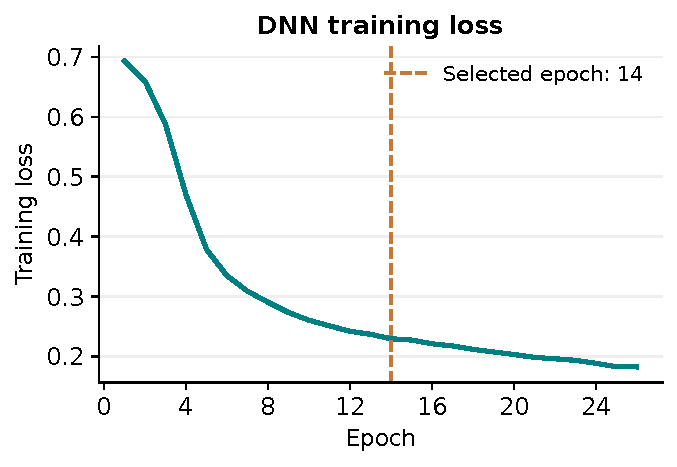
\includegraphics[width=\linewidth]{Images/09_dnn_training_loss.pdf}
\caption[DNN internal training loss]{Training loss during the internal training-length check. Lower means a better fit to training data. The dashed line marks the selected epoch 14.}
\label{fig:dnn-training-loss}
\end{minipage}\hfill
\begin{minipage}[t]{0.48\linewidth}
\vspace{0pt}
\centering
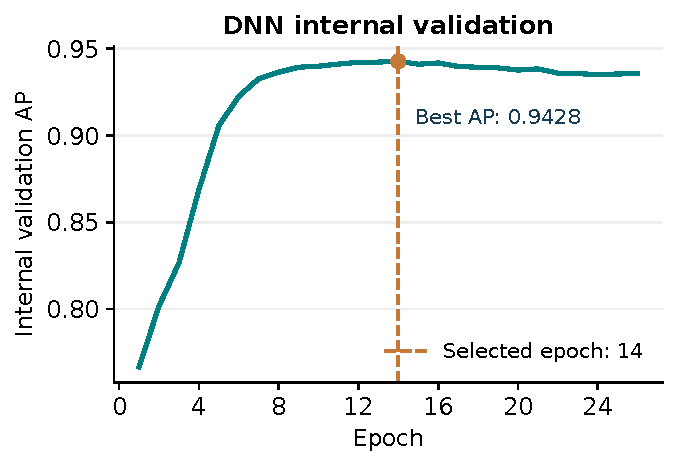
\includegraphics[width=\linewidth]{Images/09_dnn_stopping_performance.pdf}
\caption[DNN internal stopping performance]{AP for the internal validation group during the training-length check. This is one validation split, not the five-fold mean or the test score.}
\label{fig:dnn-stopping}
\end{minipage}
\end{figure}
